
%% bare_jrnl_compsoc.tex
%% V1.4b
%% 2015/08/26
%% by Michael Shell
%% See:
%% http://www.michaelshell.org/
%% for current contact information.
%%
%% This is a skeleton file demonstrating the use of IEEEtran.cls
%% (requires IEEEtran.cls version 1.8b or later) with an IEEE
%% Computer Society journal paper.
%%
%% Support sites:
%% http://www.michaelshell.org/tex/ieeetran/
%% http://www.ctan.org/pkg/ieeetran
%% and
%% http://www.ieee.org/

%%*************************************************************************
%% Legal Notice:
%% This code is offered as-is without any warranty either expressed or
%% implied; without even the implied warranty of MERCHANTABILITY or
%% FITNESS FOR A PARTICULAR PURPOSE! 
%% User assumes all risk.
%% In no event shall the IEEE or any contributor to this code be liable for
%% any damages or losses, including, but not limited to, incidental,
%% consequential, or any other damages, resulting from the use or misuse
%% of any information contained here.
%%
%% All comments are the opinions of their respective authors and are not
%% necessarily endorsed by the IEEE.
%%
%% This work is distributed under the LaTeX Project Public License (LPPL)
%% ( http://www.latex-project.org/ ) version 1.3, and may be freely used,
%% distributed and modified. A copy of the LPPL, version 1.3, is included
%% in the base LaTeX documentation of all distributions of LaTeX released
%% 2003/12/01 or later.
%% Retain all contribution notices and credits.
%% ** Modified files should be clearly indicated as such, including  **
%% ** renaming them and changing author support contact information. **
%%*************************************************************************


% *** Authors should verify (and, if needed, correct) their LaTeX system  ***
% *** with the testflow diagnostic prior to trusting their LaTeX platform ***
% *** with production work. The IEEE's font choices and paper sizes can   ***
% *** trigger bugs that do not appear when using other class files.       ***                          ***
% The testflow support page is at:
% http://www.michaelshell.org/tex/testflow/


\documentclass[10pt,journal,compsoc]{IEEEtran}
%
% If IEEEtran.cls has not been installed into the LaTeX system files,
% manually specify the path to it like:
% \documentclass[10pt,journal,compsoc]{../sty/IEEEtran}





% Some very useful LaTeX packages include:
% (uncomment the ones you want to load)


% *** MISC UTILITY PACKAGES ***
%
%\usepackage{ifpdf}
% Heiko Oberdiek's ifpdf.sty is very useful if you need conditional
% compilation based on whether the output is pdf or dvi.
% usage:
% \ifpdf
%   % pdf code
% \else
%   % dvi code
% \fi
% The latest version of ifpdf.sty can be obtained from:
% http://www.ctan.org/pkg/ifpdf
% Also, note that IEEEtran.cls V1.7 and later provides a builtin
% \ifCLASSINFOpdf conditional that works the same way.
% When switching from latex to pdflatex and vice-versa, the compiler may
% have to be run twice to clear warning/error messages.






% *** CITATION PACKAGES ***
%
%\ifCLASSOPTIONcompsoc
  % IEEE Computer Society needs nocompress option
  % requires cite.sty v4.0 or later (November 2003)
%  \usepackage[nocompress]{cite}
%\else
  % normal IEEE
\usepackage{cite}
%\fi
% cite.sty was written by Donald Arseneau
% V1.6 and later of IEEEtran pre-defines the format of the cite.sty package
% \cite{} output to follow that of the IEEE. Loading the cite package will
% result in citation numbers being automatically sorted and properly
% "compressed/ranged". e.g., [1], [9], [2], [7], [5], [6] without using
% cite.sty will become [1], [2], [5]--[7], [9] using cite.sty. cite.sty's
% \cite will automatically add leading space, if needed. Use cite.sty's
% noadjust option (cite.sty V3.8 and later) if you want to turn this off
% such as if a citation ever needs to be enclosed in parenthesis.
% cite.sty is already installed on most LaTeX systems. Be sure and use
% version 5.0 (2009-03-20) and later if using hyperref.sty.
% The latest version can be obtained at:
% http://www.ctan.org/pkg/cite
% The documentation is contained in the cite.sty file itself.
%
% Note that some packages require special options to format as the Computer
% Society requires. In particular, Computer Society  papers do not use
% compressed citation ranges as is done in typical IEEE papers
% (e.g., [1]-[4]). Instead, they list every citation separately in order
% (e.g., [1], [2], [3], [4]). To get the latter we need to load the cite
% package with the nocompress option which is supported by cite.sty v4.0
% and later. Note also the use of a CLASSOPTION conditional provided by
% IEEEtran.cls V1.7 and later.

\renewcommand{\footnoterule}
    {\noindent\smash{\rule[3pt]{8.95cm}{0.4pt}}}
    
\renewcommand{\figurename}{Figure.}
% *** GRAPHICS RELATED PACKAGES ***
%
\ifCLASSINFOpdf
   \usepackage{float}
   \usepackage[pdftex]{graphicx}
   \usepackage[%  
    colorlinks=true,
    pdfborder={0 0 0},
    linkcolor=red
    ]{hyperref}
  % declare the path(s) where your graphic files are
   \graphicspath{{../pdf/}{./png/}}
  % and their extensions so you won't have to specify these with
  % every instance of \includegraphics
  % \DeclareGraphicsExtensions{.pdf,.jpeg,.png}
\else
  % or other class option (dvipsone, dvipdf, if not using dvips). graphicx
  % will default to the driver specified in the system graphics.cfg if no
  % driver is specified.
  % \usepackage[dvips]{graphicx}
  % declare the path(s) where your graphic files are
  % \graphicspath{{../eps/}}
  % and their extensions so you won't have to specify these with
  % every instance of \includegraphics
  % \DeclareGraphicsExtensions{.eps}
\fi
% graphicx was written by David Carlisle and Sebastian Rahtz. It is
% required if you want graphics, photos, etc. graphicx.sty is already
% installed on most LaTeX systems. The latest version and documentation
% can be obtained at: 
% http://www.ctan.org/pkg/graphicx
% Another good source of documentation is "Using Imported Graphics in
% LaTeX2e" by Keith Reckdahl which can be found at:
% http://www.ctan.org/pkg/epslatex
%
% latex, and pdflatex in dvi mode, support graphics in encapsulated
% postscript (.eps) format. pdflatex in pdf mode supports graphics
% in .pdf, .jpeg, .png and .mps (metapost) formats. Users should ensure
% that all non-photo figures use a vector format (.eps, .pdf, .mps) and
% not a bitmapped formats (.jpeg, .png). The IEEE frowns on bitmapped formats
% which can result in "jaggedy"/blurry rendering of lines and letters as
% well as large increases in file sizes.
%
% You can find documentation about the pdfTeX application at:
% http://www.tug.org/applications/pdftex






% *** MATH PACKAGES ***
%
\usepackage{amsmath,amssymb}
\DeclareMathOperator*{\E}{\mathbb{E}}
% A popular package from the American Mathematical Society that provides
% many useful and powerful commands for dealing with mathematics.
%
% Note that the amsmath package sets \interdisplaylinepenalty to 10000
% thus preventing page breaks from occurring within multiline equations. Use:
%\interdisplaylinepenalty=2500
% after loading amsmath to restore such page breaks as IEEEtran.cls normally
% does. amsmath.sty is already installed on most LaTeX systems. The latest
% version and documentation can be obtained at:
% http://www.ctan.org/pkg/amsmath





% *** SPECIALIZED LIST PACKAGES ***
%
%\usepackage{algorithmic}
% algorithmic.sty was written by Peter Williams and Rogerio Brito.
% This package provides an algorithmic environment fo describing algorithms.
% You can use the algorithmic environment in-text or within a figure
% environment to provide for a floating algorithm. Do NOT use the algorithm
% floating environment provided by algorithm.sty (by the same authors) or
% algorithm2e.sty (by Christophe Fiorio) as the IEEE does not use dedicated
% algorithm float types and packages that provide these will not provide
% correct IEEE style captions. The latest version and documentation of
% algorithmic.sty can be obtained at:
% http://www.ctan.org/pkg/algorithms
% Also of interest may be the (relatively newer and more customizable)
% algorithmicx.sty package by Szasz Janos:
% http://www.ctan.org/pkg/algorithmicx




% *** ALIGNMENT PACKAGES ***
%
\usepackage{array}
% Frank Mittelbach's and David Carlisle's array.sty patches and improves
% the standard LaTeX2e array and tabular environments to provide better
% appearance and additional user controls. As the default LaTeX2e table
% generation code is lacking to the point of almost being broken with
% respect to the quality of the end results, all users are strongly
% advised to use an enhanced (at the very least that provided by array.sty)
% set of table tools. array.sty is already installed on most systems. The
% latest version and documentation can be obtained at:
% http://www.ctan.org/pkg/array


% IEEEtran contains the IEEEeqnarray family of commands that can be used to
% generate multiline equations as well as matrices, tables, etc., of high
% quality.




% *** SUBFIGURE PACKAGES ***
%\ifCLASSOPTIONcompsoc
%  \usepackage[caption=false,font=footnotesize,labelfont=sf,textfont=sf]{subfig}
%\else
%  \usepackage[caption=false,font=footnotesize]{subfig}
%\fi
% subfig.sty, written by Steven Douglas Cochran, is the modern replacement
% for subfigure.sty, the latter of which is no longer maintained and is
% incompatible with some LaTeX packages including fixltx2e. However,
% subfig.sty requires and automatically loads Axel Sommerfeldt's caption.sty
% which will override IEEEtran.cls' handling of captions and this will result
% in non-IEEE style figure/table captions. To prevent this problem, be sure
% and invoke subfig.sty's "caption=false" package option (available since
% subfig.sty version 1.3, 2005/06/28) as this is will preserve IEEEtran.cls
% handling of captions.
% Note that the Computer Society format requires a sans serif font rather
% than the serif font used in traditional IEEE formatting and thus the need
% to invoke different subfig.sty package options depending on whether
% compsoc mode has been enabled.
%
% The latest version and documentation of subfig.sty can be obtained at:
% http://www.ctan.org/pkg/subfig




% *** FLOAT PACKAGES ***
%
%\usepackage{fixltx2e}
% fixltx2e, the successor to the earlier fix2col.sty, was written by
% Frank Mittelbach and David Carlisle. This package corrects a few problems
% in the LaTeX2e kernel, the most notable of which is that in current
% LaTeX2e releases, the ordering of single and double column floats is not
% guaranteed to be preserved. Thus, an unpatched LaTeX2e can allow a
% single column figure to be placed prior to an earlier double column
% figure.
% Be aware that LaTeX2e kernels dated 2015 and later have fixltx2e.sty's
% corrections already built into the system in which case a warning will
% be issued if an attempt is made to load fixltx2e.sty as it is no longer
% needed.
% The latest version and documentation can be found at:
% http://www.ctan.org/pkg/fixltx2e


%\usepackage{stfloats}
% stfloats.sty was written by Sigitas Tolusis. This package gives LaTeX2e
% the ability to do double column floats at the bottom of the page as well
% as the top. (e.g., "\begin{figure*}[!b]" is not normally possible in
% LaTeX2e). It also provides a command:
%\fnbelowfloat
% to enable the placement of footnotes below bottom floats (the standard
% LaTeX2e kernel puts them above bottom floats). This is an invasive package
% which rewrites many portions of the LaTeX2e float routines. It may not work
% with other packages that modify the LaTeX2e float routines. The latest
% version and documentation can be obtained at:
% http://www.ctan.org/pkg/stfloats
% Do not use the stfloats baselinefloat ability as the IEEE does not allow
% \baselineskip to stretch. Authors submitting work to the IEEE should note
% that the IEEE rarely uses double column equations and that authors should try
% to avoid such use. Do not be tempted to use the cuted.sty or midfloat.sty
% packages (also by Sigitas Tolusis) as the IEEE does not format its papers in
% such ways.
% Do not attempt to use stfloats with fixltx2e as they are incompatible.
% Instead, use Morten Hogholm'a dblfloatfix which combines the features
% of both fixltx2e and stfloats:
%
% \usepackage{dblfloatfix}
% The latest version can be found at:
% http://www.ctan.org/pkg/dblfloatfix




%\ifCLASSOPTIONcaptionsoff
%  \usepackage[nomarkers]{endfloat}
% \let\MYoriglatexcaption\caption
% \renewcommand{\caption}[2][\relax]{\MYoriglatexcaption[#2]{#2}}
%\fi
% endfloat.sty was written by James Darrell McCauley, Jeff Goldberg and 
% Axel Sommerfeldt. This package may be useful when used in conjunction with 
% IEEEtran.cls'  captionsoff option. Some IEEE journals/societies require that
% submissions have lists of figures/tables at the end of the paper and that
% figures/tables without any captions are placed on a page by themselves at
% the end of the document. If needed, the draftcls IEEEtran class option or
% \CLASSINPUTbaselinestretch interface can be used to increase the line
% spacing as well. Be sure and use the nomarkers option of endfloat to
% prevent endfloat from "marking" where the figures would have been placed
% in the text. The two hack lines of code above are a slight modification of
% that suggested by in the endfloat docs (section 8.4.1) to ensure that
% the full captions always appear in the list of figures/tables - even if
% the user used the short optional argument of \caption[]{}.
% IEEE papers do not typically make use of \caption[]'s optional argument,
% so this should not be an issue. A similar trick can be used to disable
% captions of packages such as subfig.sty that lack options to turn off
% the subcaptions:
% For subfig.sty:
% \let\MYorigsubfloat\subfloat
% \renewcommand{\subfloat}[2][\relax]{\MYorigsubfloat[]{#2}}
% However, the above trick will not work if both optional arguments of
% the \subfloat command are used. Furthermore, there needs to be a
% description of each subfigure *somewhere* and endfloat does not add
% subfigure captions to its list of figures. Thus, the best approach is to
% avoid the use of subfigure captions (many IEEE journals avoid them anyway)
% and instead reference/explain all the subfigures within the main caption.
% The latest version of endfloat.sty and its documentation can obtained at:
% http://www.ctan.org/pkg/endfloat
%
% The IEEEtran \ifCLASSOPTIONcaptionsoff conditional can also be used
% later in the document, say, to conditionally put the References on a 
% page by themselves.




% *** PDF, URL AND HYPERLINK PACKAGES ***
%
\usepackage{url}
% url.sty was written by Donald Arseneau. It provides better support for
% handling and breaking URLs. url.sty is already installed on most LaTeX
% systems. The latest version and documentation can be obtained at:
% http://www.ctan.org/pkg/url
% Basically, \url{my_url_here}.





% *** Do not adjust lengths that control margins, column widths, etc. ***
% *** Do not use packages that alter fonts (such as pslatex).         ***
% There should be no need to do such things with IEEEtran.cls V1.6 and later.
% (Unless specifically asked to do so by the journal or conference you plan
% to submit to, of course. )


% correct bad hyphenation here
\hyphenation{op-tical net-works semi-conduc-tor}

\begin{document}
%
% paper title
% Titles are generally capitalized except for words such as a, an, and, as,
% at, but, by, for, in, nor, of, on, or, the, to and up, which are usually
% not capitalized unless they are the first or last word of the title.
% Linebreaks \\ can be used within to get better formatting as desired.
% Do not put math or special symbols in the title.
\title{A Study on Different Types of\\ Generative Adversarial Networks}
%
%
% author names and IEEE memberships
% note positions of commas and nonbreaking spaces ( ~ ) LaTeX will not break
% a structure at a ~ so this keeps an author's name from being broken across
% two lines.
% use \thanks{} to gain access to the first footnote area
% a separate \thanks must be used for each paragraph as LaTeX2e's \thanks
% was not built to handle multiple paragraphs
%
%
%\IEEEcompsocitemizethanks is a special \thanks that produces the bulleted
% lists the Computer Society journals use for "first footnote" author
% affiliations. Use \IEEEcompsocthanksitem which works much like \item
% for each affiliation group. When not in compsoc mode,
% \IEEEcompsocitemizethanks becomes like \thanks and
% \IEEEcompsocthanksitem becomes a line break with idention. This
% facilitates dual compilation, although admittedly the differences in the
% desired content of \author between the different types of papers makes a
% one-size-fits-all approach a daunting prospect. For instance, compsoc 
% journal papers have the author affiliations above the "Manuscript
% received ..."  text while in non-compsoc journals this is reversed. Sigh.

 
\author{Arnab~Sinha~\IEEEmembership{}% <-this % stops a space
\IEEEcompsocitemizethanks{\IEEEcompsocthanksitem Arnab Sinha is a student at The LNM Institute of Information Technology, Jaipur, India, 302031.\protect\\
% note need leading \protect in front of \\ to get a newline within \thanks as
% \\ is fragile and will error, could use \hfil\break instead.
E-mail: 17ucs034@lnmiit.ac.in}}

% note the % following the last \IEEEmembership and also \thanks - 
% these prevent an unwanted space from occurring between the last author name
% and the end of the author line. i.e., if you had this:
% 
% \author{....lastname \thanks{...} \thanks{...} }
%                     ^------------^------------^----Do not want these spaces!
%
% a space would be appended to the last name and could cause every name on that
% line to be shifted left slightly. This is one of those "LaTeX things". For
% instance, "\textbf{A} \textbf{B}" will typeset as "A B" not "AB". To get
% "AB" then you have to do: "\textbf{A}\textbf{B}"
% \thanks is no different in this regard, so shield the last } of each \thanks
% that ends a line with a % and do not let a space in before the next \thanks.
% Spaces after \IEEEmembership other than the last one are OK (and needed) as
% you are supposed to have spaces between the names. For what it is worth,
% this is a minor point as most people would not even notice if the said evil
% space somehow managed to creep in.



% The paper headers
% \markboth{Journal of \LaTeX\ Class Files,~Vol.~14, No.~8, August~2015}%
% {Shell \MakeLowercase{\textit{et al.}}: Bare Demo of IEEEtran.cls for Computer Society Journals}
% The only time the second header will appear is for the odd numbered pages
% after the title page when using the twoside option.
% 
% *** Note that you probably will NOT want to include the author's ***
% *** name in the headers of peer review papers.                   ***
% You can use \ifCLASSOPTIONpeerreview for conditional compilation here if
% you desire.



% The publisher's ID mark at the bottom of the page is less important with
% Computer Society journal papers as those publications place the marks
% outside of the main text columns and, therefore, unlike regular IEEE
% journals, the available text space is not reduced by their presence.
% If you want to put a publisher's ID mark on the page you can do it like
% this:
%\IEEEpubid{0000--0000/00\$00.00~\copyright~2015 IEEE}
% or like this to get the Computer Society new two part style.
%\IEEEpubid{\makebox[\columnwidth]{\hfill 0000--0000/00/\$00.00~\copyright~2015 IEEE}%
%\hspace{\columnsep}\makebox[\columnwidth]{Published by the IEEE Computer Society\hfill}}
% Remember, if you use this you must call \IEEEpubidadjcol in the second
% column for its text to clear the IEEEpubid mark (Computer Society jorunal
% papers don't need this extra clearance.)



% use for special paper notices
%\IEEEspecialpapernotice{(Invited Paper)}



% for Computer Society papers, we must declare the abstract and index terms
% PRIOR to the title within the \IEEEtitleabstractindextext IEEEtran
% command as these need to go into the title area created by \maketitle.
% As a general rule, do not put math, special symbols or citations
% in the abstract or keywords.
\IEEEtitleabstractindextext{%
\begin{abstract}
The abstract goes here.
\end{abstract}

% Note that keywords are not normally used for peerreview papers.
\begin{IEEEkeywords}
generator, adversarial, discriminator, minimax, super-resolution
\end{IEEEkeywords}}


% make the title area
\maketitle


% To allow for easy dual compilation without having to reenter the
% abstract/keywords data, the \IEEEtitleabstractindextext text will
% not be used in maketitle, but will appear (i.e., to be "transported")
% here as \IEEEdisplaynontitleabstractindextext when the compsoc 
% or transmag modes are not selected <OR> if conference mode is selected 
% - because all conference papers position the abstract like regular
% papers do.
\IEEEdisplaynontitleabstractindextext
% \IEEEdisplaynontitleabstractindextext has no effect when using
% compsoc or transmag under a non-conference mode.



% For peer review papers, you can put extra information on the cover
% page as needed:
% \ifCLASSOPTIONpeerreview
% \begin{center} \bfseries EDICS Category: 3-BBND \end{center}
% \fi
%
% For peerreview papers, this IEEEtran command inserts a page break and
% creates the second title. It will be ignored for other modes.
\IEEEpeerreviewmaketitle



\IEEEraisesectionheading{\section{Introduction}\label{sec:introduction}}
% Computer Society journal (but not conference!) papers do something unusual
% with the very first section heading (almost always called "Introduction").
% They place it ABOVE the main text! IEEEtran.cls does not automatically do
% this for you, but you can achieve this effect with the provided
% \IEEEraisesectionheading{} command. Note the need to keep any \label that
% is to refer to the section immediately after \section in the above as
% \IEEEraisesectionheading puts \section within a raised box.




% The very first letter is a 2 line initial drop letter followed
% by the rest of the first word in caps (small caps for compsoc).
% 
% form to use if the first word consists of a single letter:
% \IEEEPARstart{A}{demo} file is ....
% 
% form to use if you need the single drop letter followed by
% normal text (unknown if ever used by the IEEE):
% \IEEEPARstart{A}{}demo file is ....
% 
% Some journals put the first two words in caps:
% \IEEEPARstart{T}{his demo} file is ....
% 
% Here we have the typical use of a "T" for an initial drop letter
% and "HIS" in caps to complete the first word.
\IEEEPARstart{D}{eep} learning has shown admirable progress over the past decade in discriminative tasks, mostly pertaining to classification of high dimensional data. However, deep generative modeling never took off similarly due to the stochasticity prevalent in the underlying probability computations, until Goodfellow et al. proposed their novel work in the form of generative adversarial networks \cite{vanillagans}. Generative adversarial networks revolves around the concept of training two models against each other, the generative model and an adversary in the form of a discriminative model. The generator focuses on creating counterfeit data while the discriminator aims at detecting the fake article correctly. This one-on-one rivalry continues till an equilibrium is reached and the discriminator is forced to randomly choose between a fake and a real output. This algorithm can help achieve several tasks that could be comparatively more expensive using methods established so far in pure discriminative modeling.

The research laid out in this report is inspired by the unprecedented success of GANs in various domains and the inquisitiveness to understand the foundation concepts underlying it. The objective was to learn about the mathematics needed to understand its working and then explore various improvisations performed on the foundational concept of GANs. My attempts to work with GANs involved testing the algorithm proposed in \cite{vanillagans} and \cite{ledig2017photo} on two and three dimensional data, much smaller compared to the image data used in original experiments. The motive behind this was to observe if the proposed algorithm produced similar results with sparse amount of features or dimensions as well. 
% You must have at least 2 lines in the paragraph with the drop letter
% (should never be an issue)

% \hfill mds
 
% \hfill August 26, 2015

% needed in second column of first page if using \IEEEpubid
%\IEEEpubidadjcol

% \subsubsection{Subsubsection Heading Here}
% Subsubsection text here.


% An example of a floating figure using the graphicx package.
% Note that \label must occur AFTER (or within) \caption.
% For figures, \caption should occur after the \includegraphics.
% Note that IEEEtran v1.7 and later has special internal code that
% is designed to preserve the operation of \label within \caption
% even when the captionsoff option is in effect. However, because
% of issues like this, it may be the safest practice to put all your
% \label just after \caption rather than within \caption{}.
%
% Reminder: the "draftcls" or "draftclsnofoot", not "draft", class
% option should be used if it is desired that the figures are to be
% displayed while in draft mode.
%
%\begin{figure}[!t]
%\centering
%\includegraphics[width=2.5in]{myfigure}
% where an .eps filename suffix will be assumed under latex, 
% and a .pdf suffix will be assumed for pdflatex; or what has been declared
% via \DeclareGraphicsExtensions.
%\caption{Simulation results for the network.}
%\label{fig_sim}
%\end{figure}

% Note that the IEEE typically puts floats only at the top, even when this
% results in a large percentage of a column being occupied by floats.
% However, the Computer Society has been known to put floats at the bottom.


% An example of a double column floating figure using two subfigures.
% (The subfig.sty package must be loaded for this to work.)
% The subfigure \label commands are set within each subfloat command,
% and the \label for the overall figure must come after \caption.
% \hfil is used as a separator to get equal spacing.
% Watch out that the combined width of all the subfigures on a 
% line do not exceed the text width or a line break will occur.
%
%\begin{figure*}[!t]
%\centering
%\subfloat[Case I]{\includegraphics[width=2.5in]{box}%
%\label{fig_first_case}}
%\hfil
%\subfloat[Case II]{\includegraphics[width=2.5in]{box}%
%\label{fig_second_case}}
%\caption{Simulation results for the network.}
%\label{fig_sim}
%\end{figure*}
%
% Note that often IEEE papers with subfigures do not employ subfigure
% captions (using the optional argument to \subfloat[]), but instead will
% 
% /describe all of them (a), (b), etc., within the main caption.
% Be aware that for subfig.sty to generate the (a), (b), etc., subfigure
% labels, the optional argument to \subfloat must be present. If a
% subcaption is not desired, just leave its contents blank,
% e.g., \subfloat[].


% An example of a floating table. Note that, for IEEE style tables, the
% \caption command should come BEFORE the table and, given that table
% captions serve much like titles, are usually capitalized except for words
% such as a, an, and, as, at, but, by, for, in, nor, of, on, or, the, to
% and up, which are usually not capitalized unless they are the first or
% last word of the caption. Table text will default to \footnotesize as
% the IEEE normally uses this smaller font for tables.
% The \label must come after \caption as always.
%
%\begin{table}[!t]
%% increase table row spacing, adjust to taste
%\renewcommand{\arraystretch}{1.3}
% if using array.sty, it might be a good idea to tweak the value of
% \extrarowheight as needed to properly center the text within the cells
%\caption{An Example of a Table}
%\label{table_example}
%\centering
%% Some packages, such as MDW tools, offer better commands for making tables
%% than the plain LaTeX2e tabular which is used here.
%\begin{tabular}{|c||c|}
%\hline
%One & Two\\
%\hline
%Three & Four\\
%\hline
%\end{tabular}
%\end{table}


% Note that the IEEE does not put floats in the very first column
% - or typically anywhere on the first page for that matter. Also,
% in-text middle ("here") positioning is typically not used, but it
% is allowed and encouraged for Computer Society conferences (but
% not Computer Society journals). Most IEEE journals/conferences use
% top floats exclusively. 
% Note that, LaTeX2e, unlike IEEE journals/conferences, places
% footnotes above bottom floats. This can be corrected via the
% \fnbelowfloat command of the stfloats package.
\begin{figure*}
    \centering
    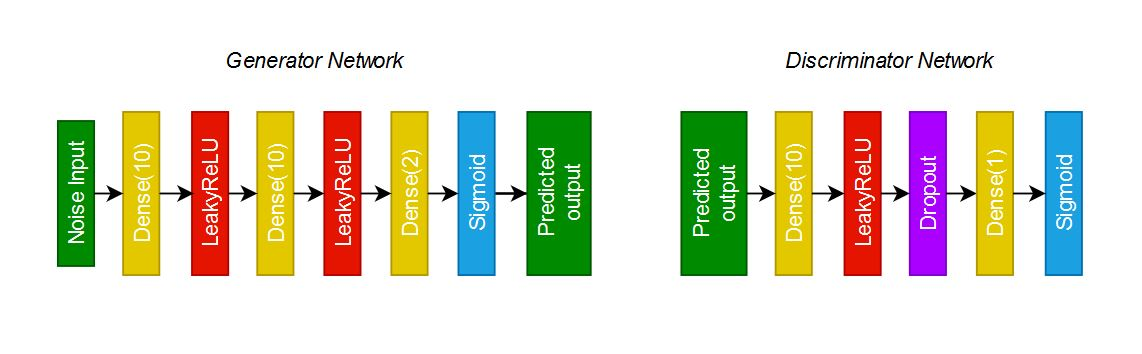
\includegraphics[scale = 1.5, height = 4cm, width = 14cm]{gans600}
    \caption{A general overview of the network architecture used for the experiments on Vanilla GANs and SRGANs.}
    \label{fig:gansfig}
\end{figure*}

\section{Method}

During the course of this internship, I learnt about and explored three types of GAN variations: Vanilla GANs , Super Resolution GANs and Conditional GANs. The following
section shall focus upon the mathematics underlying these novel models.

\subsection{Vanilla GANs}
The preliminary version of generative adversarial networks is pretty straightforward and easy to understand. The fact that it was implemented with simple multilayer perceptrons made it easier to generate an intuition behind it. It focuses on creating a mapping, \textit{G(\textbf{z}; $\theta$\textsubscript{g})}  $\rightarrow$ \textbf{\textit{y}}, from an input vector \textbf{\textit{z}}, belonging to a prior distribution  \textit{p\textsubscript{z}}, to an output image \textbf{\textit{y}}. \textit{G} is a differentiable function represented by the multilayer perceptron with \textit{$\theta$\textsubscript{g}} as parameters of neural network. The final theoretical aim is to make \textit{p\textsubscript{data}} = \textit{p\textsubscript{g}}, where \textit{p\textsubscript{data}} corresponds the probability distribution of the true data whereas  \textit{p\textsubscript{g}} corresponds to the probability distribution of the data generated by the Generator \textit{G}. A second multilayer perceptron, the opposition network, called the Discriminator, \textit{D(\textbf{x}; $\theta$\textsubscript{d})}, is defined, where, for \textbf{x} $\sim$ \textit{p\textsubscript{data}}, D(\textbf{x}) is the probability of \textbf{x} belonging to \textit{p\textsubscript{data}} rather than \textit{p\textsubscript{g}}. We train \textit{D} to maximize this probability by training the actual data and generated data with their respective correct labels, 1 for real images and 0 for fake images. We simultaneously train \textit{G} to minimize the probability of $\log(1- \textit{D}(\textit{G}(\textbf{z})))$. The entire equation goes as follows:%
\begin{multline}
\mathop{min}_{G}\; \mathop{max}_{D}\; \mbox{V}(G,D)\; \mbox{E}_{\textbf{x}\sim p_{data}(\textbf{x})} \log[D(\textbf{x})]\\
+ \mbox{E}_{\textbf{z}\sim p_{z}(\textbf{z})} \log[1 - \textit{D}({\textit{G}}(\textbf{z}))]
\end{multline}
The process is an iterative and numerical one, as mentioned by Goodfellow et al. in \cite{vanillagans}, where, for every \textit{k} iterations of discriminator training, 1 iteration of generator training is implemented. This ensures optimality of the discriminator and slow training of the generator. However, it has been observed and recommended to maximize $\log(\textit{D}(\textit{G}(\textbf{z})))$ rather than minimizing $\log(1- \textit{D}(\textit{G}(\textbf{z})))$ proves beneficial as the latter does not produce sufficient gradients in the initial stages of training in order to train \textit{G} well.

\subsection{Super Resolution GANs}
GANs finds its applications in image super resolution as well. Convolutional neural networks have proven to give supreme results \cite{lecun2015lenet,krizhevsky2012imagenet,simonyan2014very} in the past with image related tasks and it is no different here as well. Ledig et al. in \cite{ledig2017photo} have described both the generator and discriminator to be convolutional networks, with the core of the ResNet architecture \cite{he2016deep}. The two networks, combined, attempt to create a mapping, \textit{G}(\textbf{x\textsuperscript{LR}}; $\theta$\textsubscript{g}) $\rightarrow$ \textbf{x\textsuperscript{HR}}, where \textbf{x}\textsuperscript{LR} $\sim$ \textit{p}\textsuperscript{LR}, the probability distribution of low resolution images, \textbf{x}\textsuperscript{HR} $\sim$  \textit{p}\textsuperscript{HR}, the probability distribution of actual high resolution images, and \textit{$\theta$\textsubscript{g}} defines the parameters of \textit{G}. In totality, a minimax game is played, which can be mathematically presented as follows:%
\begin{multline}
\mathop{min}_{G}\; \mathop{max}_{D}\; \mbox{V}(G,D)\; \mbox{E}_{\textbf{x}^{HR}\sim p^{HR}} \log[D(\textbf{x}^{HR})]\\
+ \mbox{E}_{\textbf{x}^{LR}\sim p^{LR}} \log[1 - \textit{D}({\textit{G}}(\textbf{x}^{LR}))]
\end{multline}
The discriminator \textit{D} is trained so as to resolve the conflict between super resolved images and real high resolution images. The generator, on the other hand, has a slightly modified loss function, called perceptual loss. While the generative adversarial loss stays the same as in Vanilla GANs, an additional content loss is added. The content loss is derived from pixel-wise MSE loss. The latter uses absolute values of the pixel intensities, whereas the content loss uses values from the ReLU activation layers of a pre-trained VGG19 network as described in \cite{simonyan2014very}. The loss is defined as the euclidean distance between the feature map values of the super-resolved image $\textit{G}(\textbf{x}^{LR})$ and the real image $\textbf{x}^{HR}$. The content loss formula cited from \cite{ledig2017photo} goes as follows:
\begin{multline}
l^{SR}_{VGG/i,j} = \frac{1}{W_{i,j}H_{i,j}} \sum_{x=1}^{W_{i,j}} \sum_{y=1}^{H_{i,j}} ( \phi_{i,j}(I^{HR})_{x,y} -\\
\phi_{i,j}(G_{\theta_{G}}(I^{LR}))_{x,y})^{2}
\end{multline}
Here, $W_{i,j}$ and $H_{i,j}$ are the width and height of $\phi_{i,j}$, the feature map obtained after the j-th convolution, post activation, before the i-th max pooling layer within the VGG19 network.  Following this, the total perceptual loss, also cited from \cite{ledig2017photo}, takes the following form:
\begin{align}
\label{eq4}
l^{SR}& = \underbrace{l_{X}^{SR}}_\text{content loss} + \underbrace{\lambda l_{Gen}^{SR}}_\text{adversarial loss}
\end{align}
where \(l_{Gen}^{SR} = \sum_{n-1}^{N} -\log D_{\theta_{D}}(G_{\theta_{G}}(I^{LR}))\), concurring with the observation laid out by Goodfellow et al. in \cite{vanillagans}, where minimizing over \(-\log D_{\theta_{D}}(G_{\theta_{G}}(I^{LR}))\), proves to give better results compared to minimizing over \(\log[1- D_{\theta_{D}}(G_{\theta_{G}}(I^{LR}))]\). However, in my experiments, due to the type of dataset used, I have used element-wise MSE loss instead of the above described content loss.

\subsection{Network Architecture}
A common internal architecture for the generator and discriminator was used for both the experiments. As illustrated in Figure \ref{fig:gansfig}, the generator consists of two hidden dense layers with Leaky ReLU activation functions, followed by another dense layer with a sigmoid activation function. Comparatively worse results were observed if the generator included a single hidden dense layer, thereby concluding that a more powerful generator was needed. On the other hand, a single hidden dense layer, with Leaky ReLU activation and dropout, was found to be sufficient for the discriminator. Leaky ReLU was implemented as an improvisation to the work by Glorot et al. in \cite{glorot2011deep}. Following the work proposed by Srivastava et al. in \cite{srivastava2014dropout}, dropout was used as a regularization method to train the discriminator in a way that it could perform optimally on unseen data as well. The only difference, with respect to the networks used in the two experiments, is that the size of the predicted output was taken to be 2 for Vanilla GANs and 3 for SRGANs.

\section{Experiments}

\subsection{Dataset}\label{Sec31}
For the Vanilla GANs experiment, a 2-dimensional dataset of 1500 points, with mean values at (1,1), (6,6), (11,11) and standard deviation values (0.5,0.5), (0.6,0.6), (1,1) was used. Moving on, in the SRGANs experiment, a 2-dimensional dataset with mean values (20,20), (40,40), (80,80) and standard deviation values (1,1), (3,3), (5,5) has been used for the low dimensional input to the generator. To replicate the actual high dimensional input to the discriminator, a 3-dimensional dataset with the $3^{rd}$ dimension \(z = 0.25*x + 0.75*y\) was used. All the data points were sampled from a multivariate Gaussian distribution with means and standard deviations taken as mentioned above for the respective experiments.

\begin{figure*}[t]
\subfloat{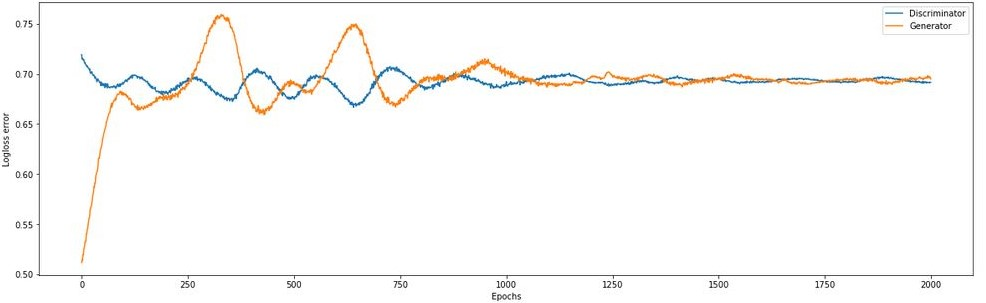
\includegraphics[width=4.7in,height=1.55in]{error_graph_trimodal600}}
\quad\quad\hspace{-6pt}
\subfloat{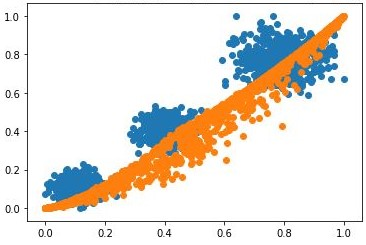
\includegraphics[width=2.2in,height=1.55in]{trimodal_data_comparison600}}
\hfil
\subfloat{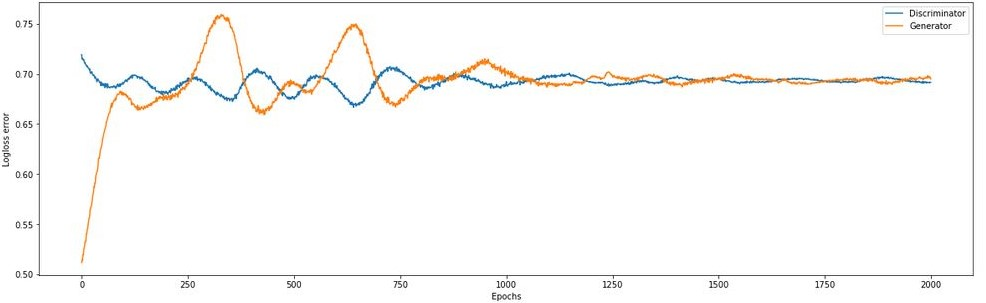
\includegraphics[width=4.7in,height=1.55in]{error_graph_trimodal600}}
\quad\quad\hspace{-6pt}
\subfloat{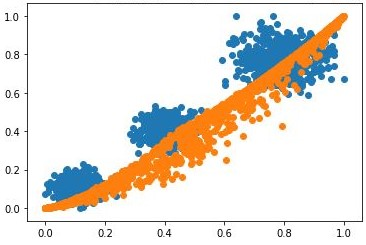
\includegraphics[width=2.2in,height=1.55in]{trimodal_data_comparison600}}
\caption{(Top Left)Training log-loss error graph for generator(in orange) and discriminator(in blue) spanning 2000 epochs in Vanilla GANs experiment,  (Top Right)Training dataset(in blue) for Vanilla GANs experiment and predicted set of 1500 points(in orange) by generator after training,(Bottom Left)Training log-loss error graph for generator(in orange) and discriminator(in blue) spanning 2000 epochs in SRGANs experiment,  (Bottom Right)Training dataset(in blue) for SRGANs experiment and predicted set of 600 points(in orange) by generator after training}
\label{data1}
\end{figure*}

\subsection{Training}
The training was performed on an NVIDIA GeForce 940MX GPU using the dataset described in section \ref{Sec31}. For Vanilla GANs, the training dataset itself was used for testing. As a pre-processing step, the data points were normalized to a scale of [0,1] before feeding into the model. For optimization we use Adam \cite{kingma2014adam} with $\beta_{1}$ = 0.9 and $\beta_{2}$ = 0.999. The mini-batch size was set to 100. For faster convergence, the learning rate was set to 10$^{-2}$ in the first 1000 epochs and reduced to 2*10$^{-4}$ for the next 1000 to maintain stability. 

In the next experiment pertaining to SRGANs, a separate dataset of 600 points with identical statistics as that of the training data, was used. The pre-processing steps and optimizers used here are identical to that followed in the Vanilla GANs experiment. The mini-batch size is set to 200. Several runs of the model were performed for different values of $\lambda$ while keeping the seed value constant to nullify randomness in every run. All the variants were trained with 500 epochs at a learning rate of 10$^{-4}$ and another 500 epochs with a learning rate of 10$^{-3}$. The discriminator and generator are trained alternately, which is identical to using \textit{k} = 1 as used in Goodfellow et al. \cite{vanillagans}. The implementation was done using Pytorch framework and can be found on GitHub\footnote{\url{https://github.com/arnabsinha99/GANs}}.

\

\renewcommand{\arraystretch}{1.5}
\begin{table}[h]
\begin{center}
\begin{tabular}{|c|c|}
\hline
Lambda ($\lambda$)&   MSE value\\
\hline
0& 4.6596 * 1e-5\\
\hline
0.00001& 4.6596 * 1e-5\\
\hline
0.0001& 4.6596 * 1e-5\\
\hline
0.001& 4.6596 * 1e-5\\
\hline
0.01& 4.6596 * 1e-5\\
\hline
0.1& 4.6596 * 1e-5\\
\hline
0.125& 4.6596 * 1e-5\\
\hline
0.25& 4.6596 * 1e-5\\
\hline
0.5& 4.6596 * 1e-5\\
\hline
\textbf{1}& \textbf{4.6596} * \textbf{1e-5}\\
\hline
1.5& 4.6596 * 1e-5\\
\hline
2& 4.6596 * 1e-5\\
\hline
10& 4.6596 * 1e-5\\
\hline
\end{tabular}
\end{center}
\caption{Comparison of different values of $\lambda$ used in equation \ref{eq4} with the help of Mean Squared Error values on the test dataset for a single run}
\label{table1}
\end{table}
\subsection{Investigation on content loss}
In the work put forward by Ledig et al. \cite{ledig2017photo}, the value of $\lambda$ has been used as 10$^{-3}$. However, parameters are always application dependent and therefore several runs were performed to find an approximately optimal value for $\lambda$ used in equation \ref{eq4}. A different result was observed as laid out in Table \ref{table1}. The MSE value is the least for $\lambda$ = 1, which is different from the value used in the actual SRGAN experiments conducted by Ledig et al. \cite{ledig2017photo}. A steady rise is observed when using values above 1 whereas an overall increase with minor fluctutations were seen for values below 1 upto 0. 

\section{Conclusion and Future Scope}






% if have a single appendix:
%\appendix[Proof of the Zonklar Equations]
% or
%\appendix  % for no appendix heading
% do not use \section anymore after \appendix, only \section*
% is possibly needed

% use appendices with more than one appendix
% then use \section to start each appendix
% you must declare a \section before using any
% \subsection or using \label (\appendices by itself
% starts a section numbered zero.)
%

% \appendices
% \section{Proof of the First Zonklar Equation}
% Appendix one text goes here.

% % you can choose not to have a title for an appendix
% % if you want by leaving the argument blank
% \section{}
% \vspace{100pt}
% Appendix two text goes here.


% % use section* for acknowledgment
% \ifCLASSOPTIONcompsoc
%   % The Computer Society usually uses the plural form
%   \section*{Acknowledgments}
% \else
%   % regular IEEE prefers the singular form
%   \section*{Acknowledgment}
% \fi


% The authors would like to thank...


% Can use something like this to put references on a page
% by themselves when using endfloat and the captionsoff option.
\ifCLASSOPTIONcaptionsoff
  \newpage
\fi



% trigger a \newpage just before the given reference
% number - used to balance the columns on the last page
% adjust value as needed - may need to be readjusted if
% the document is modified later
%\IEEEtriggeratref{8}
% The "triggered" command can be changed if desired:
%\IEEEtriggercmd{\enlargethispage{-5in}}

% references section

% can use a bibliography generated by BibTeX as a .bbl file
% BibTeX documentation can be easily obtained at:
% http://mirror.ctan.org/biblio/bibtex/contrib/doc/
% The IEEEtran BibTeX style support page is at:
% http://www.michaelshell.org/tex/ieeetran/bibtex/
%\bibliographystyle{IEEEtran}
% argument is your BibTeX string definitions and bibliography database(s)
%\bibliography{IEEEabrv,../bib/paper}
%
% <OR> manually copy in the resultant .bbl file
% set second argument of \begin to the number of references
% (used to reserve space for the reference number labels box)
\bibliographystyle{IEEEtran}
\bibliography{IEEEabrv,sample}
% if you will not have a photo at all:
% \begin{IEEEbiographynophoto}{John Doe}
% Biography text here.
% \end{IEEEbiographynophoto}

% insert where needed to balance the two columns on the last page with
% biographies
%\newpage

% \begin{IEEEbiographynophoto}{Jane Doe}
% Biography text here.
% \end{IEEEbiographynophoto}

% You can push biographies down or up by placing
% a \vfill before or after them. The appropriate
% use of \vfill depends on what kind of text is
% on the last page and whether or not the columns
% are being equalized.

%\vfill

% Can be used to pull up biographies so that the bottom of the last one
% is flush with the other column.
%\enlargethispage{-5in}



% that's all folks
\end{document}


